\documentclass{article}
\usepackage[utf8]{inputenc}
\usepackage{graphicx}
\usepackage{float}
\graphicspath{ {img/} }
\begin{document}

\title{GroundsBot:Autonomous Golf Course Maintenance}
\date{September 2017}
\author{Team A        \\ David Evans \\
        Adam Driscoll \\ Henry Chen  \\
        Josh Bennett  \\ Joe Phaneuf \\ }
\maketitle
\newpage

\tableofcontents
\newpage

\section{Project Description}
GroundsBot \\
\subsection{Functional Requirements}
Groundsbot shall:
  Receive mowing regions
  Cut grass at the correct height
  Create a mowing plan
  Cut the rough 
  Avoid obstacles
  Provide feedback to the groundskeeper
\begin{center}
\begin{tabular}{ |c|c|c| }
  \hline
    M.P1 & Req 1 & My First Requirement \\
    D.P1 & Req 2 & My Second Requirement \\
  \hline
\end{tabular}
\end{center}

\subsection{Non-Functional Requirements}
M.N.1 Bot has emergency stop \\
M.N.2 Bot is clearly visible/noticeable \\
M.N.3 Bot does not destroy grass \\
D.N.1 Operates in variable lighting conditions \\
D.N.2 Deck adjustable 0.5” to 2” \\
D.N.3 Survives deluge of golf balls \\


\subsection{Performance Requirements}
M.P.1 First time user inputs map within 15 minutes \\
M.P.2 System returns proposed route/coverage map within 5 minutes \\
M.P.3 Cut 0-25\% overlap for 95\% of grass \\
M.P.4 Mow 50 $ft^2$ of 30 degree sloped grass \\
M.P.5 Detect 80\% of objects greater than 27 cubic inches \\
M.P.6 Mow to within 1 foot of detected obstacles \\
M.P.7 Mow 90\% of a $\frac{1}{4}$ acre area \\

\noindent
D.P.1 Mow to within 3 inches of a detected obstacles \\
D.P.2 Return home to within 5 feet of start \\
D.P.2+ Return home to and mates with a charging dock \\
D.P.3 Visually report mowing mowing coverage and known obstacles \\

\section{Use Case}

\section{System Level Requirements}
Objective Tree
Work with existing operations
  Minimal installation effort
  Operate with minimal intervention
  Allow for machine maintenance

Upholds golf course standards
  Operates safely 
  Reflects golfing aesthetics
  Low impact on golfers
  
Reduce net rough maintenance cost
  Reduce manual labor
  Reduce ammmortized cost per acre
  
\subsection{Chassis and Drivetrain}
\subsection{Sensor Suite}

\section{Functional Architecture}
\begin{figure}[H]
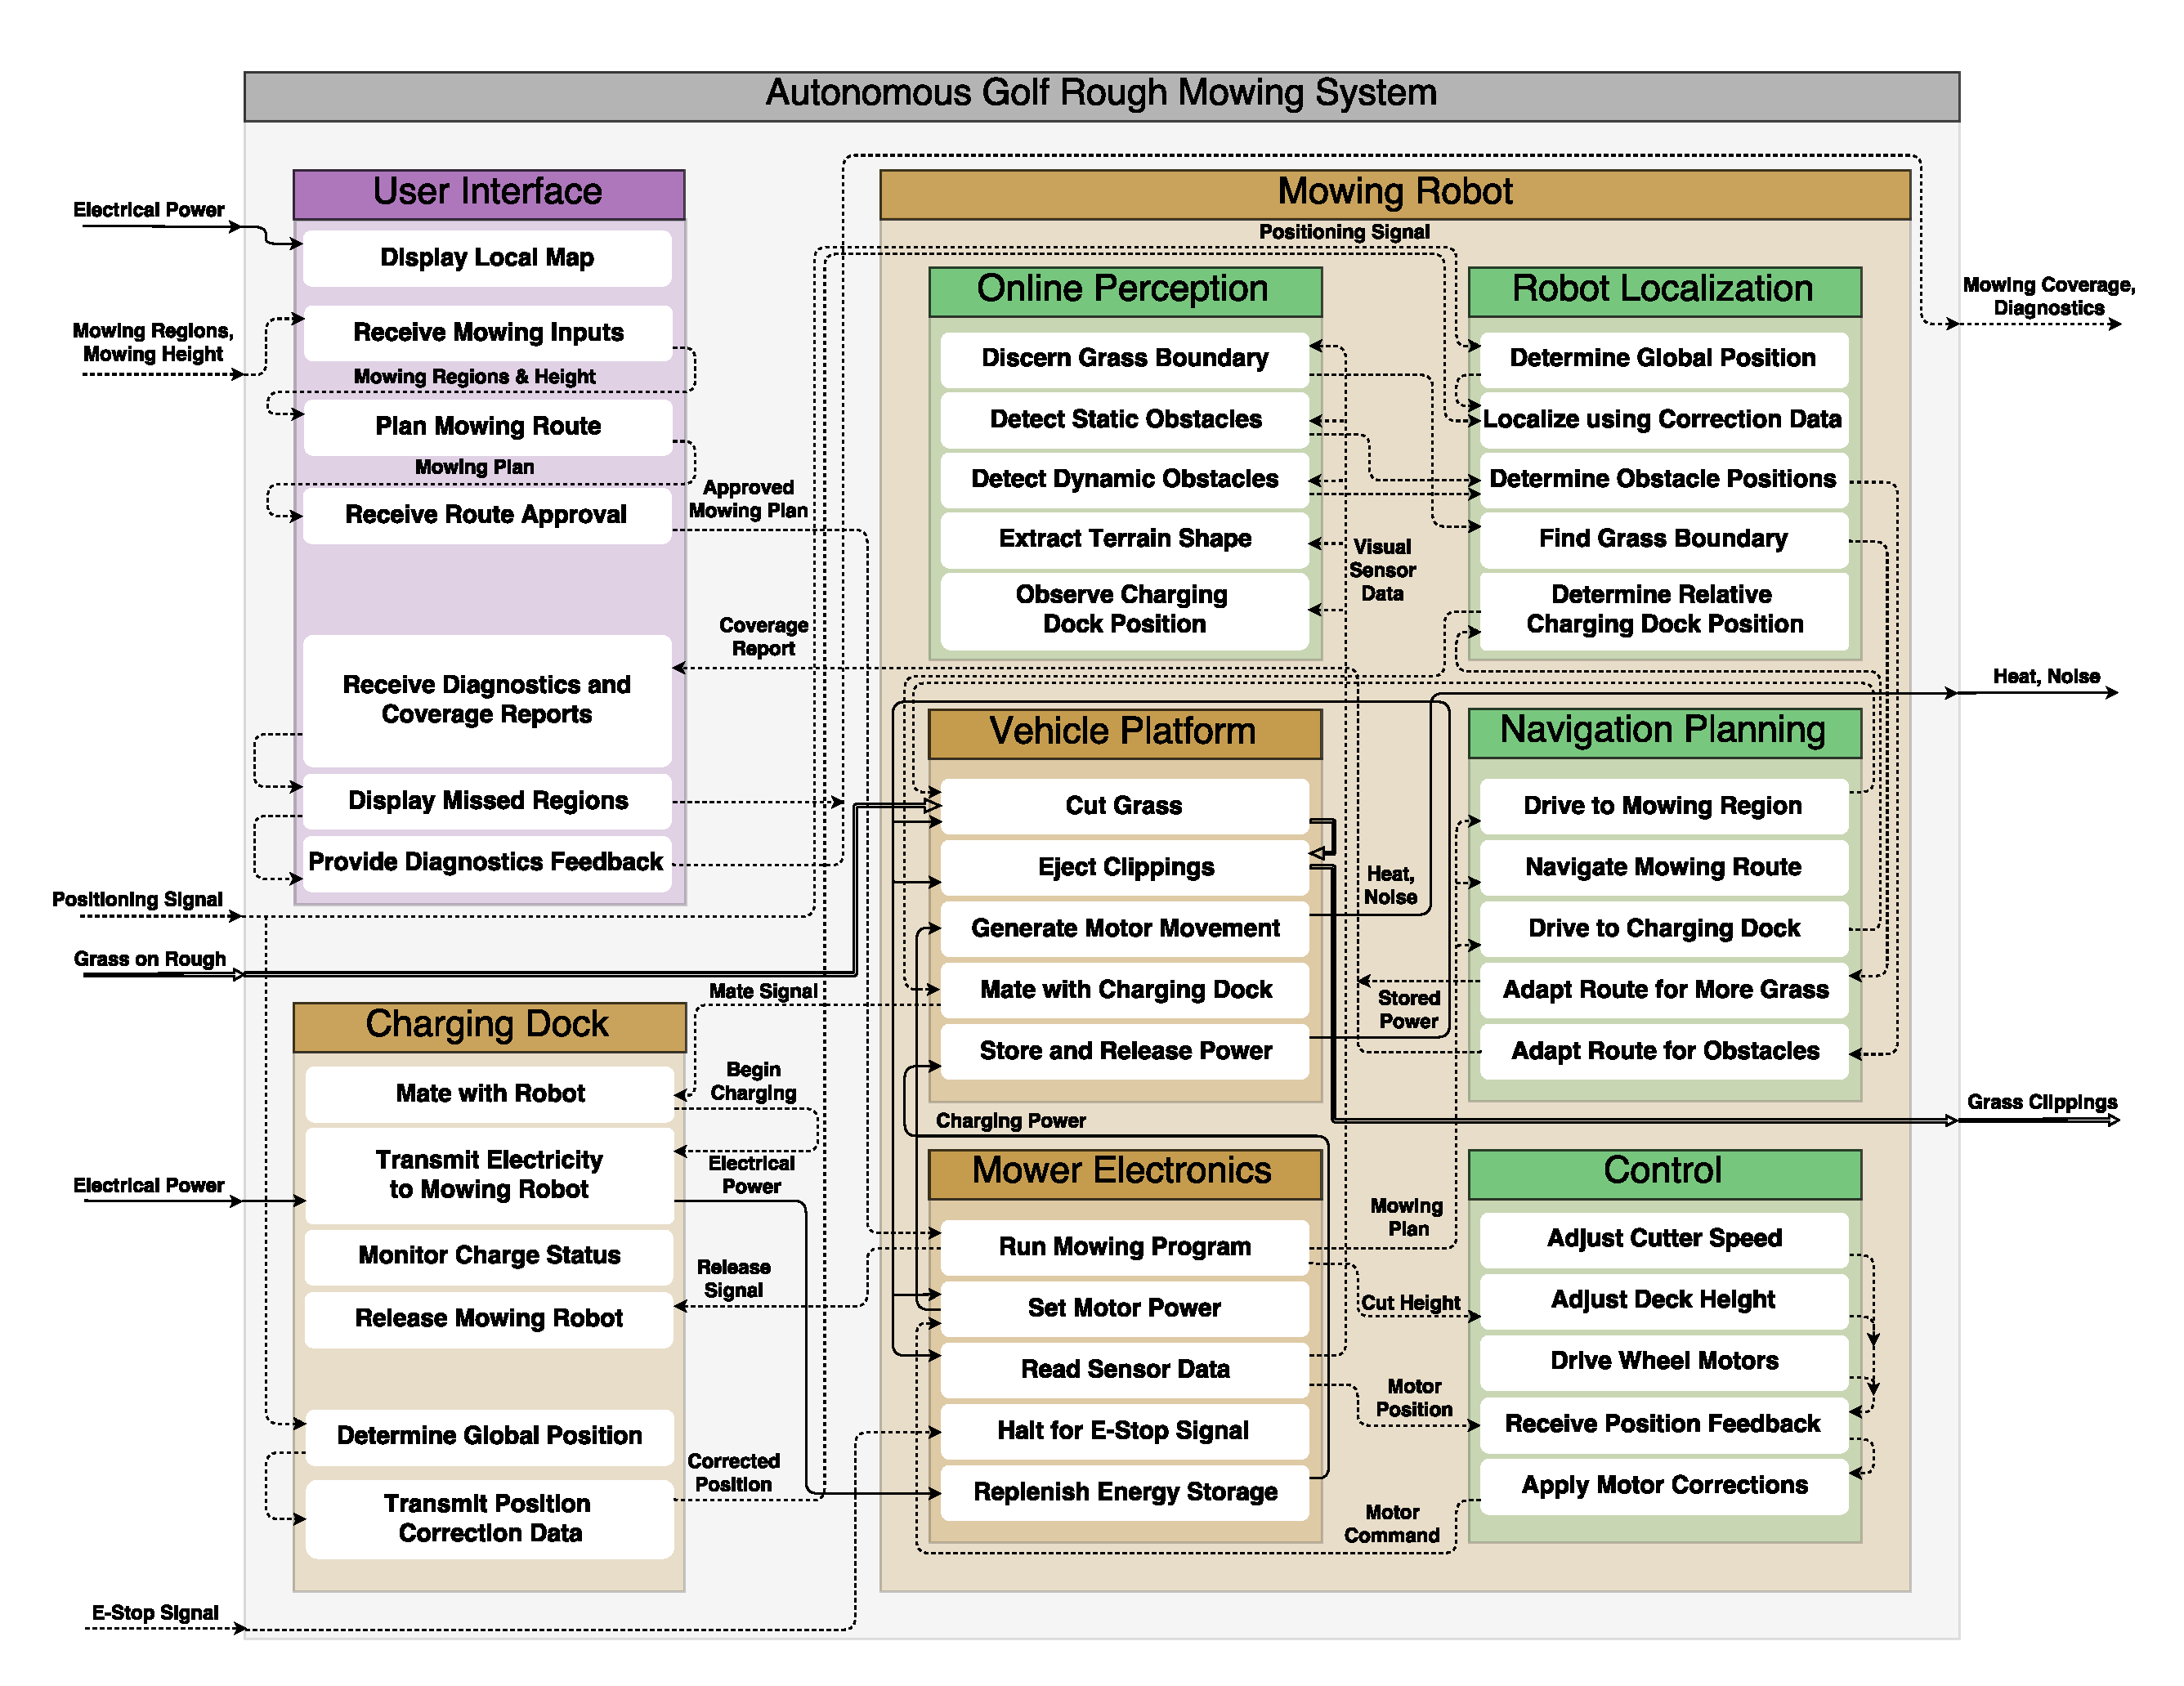
\includegraphics[scale=0.3]{functional}
\caption{Functional Architecture}
\label{fig:functional}
\end{figure}


\section{System Level Trade Studies}

\section{Cyberphysical Architecture}
\begin{figure}[H]
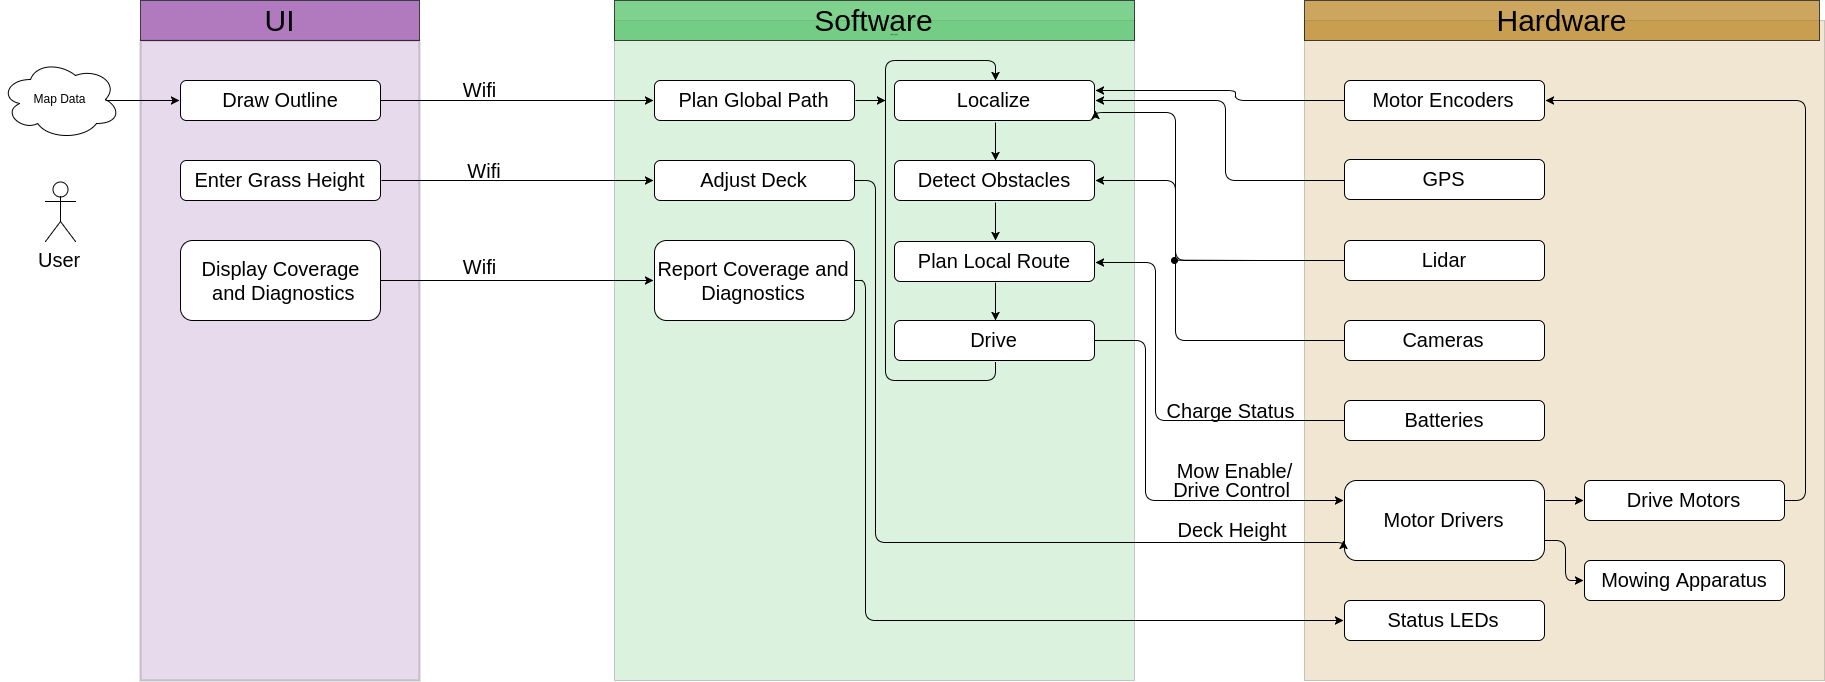
\includegraphics[scale=0.2]{cyberphysical}
\caption{Cyberphysical Architecture}
\label{fig:cyberphysical}
\end{figure}

  The user interface and IO subsystems are the contact points for the operator.  The wifi access point allows the user to load mowing boundaries from their laptop or mobile device.  This also enables the user to download coverage reports and diagnostics.  Status LEDs allow the operator to understand the system status at a glance, while safety beacons alert humans to GroundsBot's presence at a distance. \\

  GroundsBot uses its sensor suite to ensure a clean cut. GPS, IMU, and Motor Encoders are used for coarse localization while the cameras are used to ensure optimal grass overlap while cutting.  Cameras and lidar also enable GroundsBot to detect static and dynamic obstacles.\\

  GroundsBot's battery subsystem reports charge status to the CPU to prevent GroundsBot from becoming stranded. The battery subsystem also contains standard protection protocols including charge control, under-voltage lockout, and over-current protection. \\

  The CPU utilizes sensor information for localization, obstacle detection, and planning.  After a local path is devised drive signals are sent to the motors. The CPU also logs coverage data and generates reports.\\

  The Drive Train contains motors and motor drivers to propel GroundsBot across a golf course.  This also encompasses the mowing apparatus and mowing deck height control. \\



\section{Subsystem Descriptions}
	\subsection{UI}
	An important aspect of the project is a way for the user to communicate his desired mowing path to the robot. This input method must be separate from the robot itself, allowing the user to be somewhere else as the robot mows autonomously. 
	
	This will be achieved through a mobile device, either a dedicated tablet or the user's own smartphone. An app or website will be loaded onto this device, and allow for the user to input a map outline that will be communicated to the robot. 
	
	\subsection{Hardware}
		\subsubsection{Platform}
		TODO: FINISH THIS PART - dependent on trade study \\ 
			The powertrain will consist of electric drive motors and batteries obtained from the sponsor. 
			
		\subsubsection{Mower}
			In addition to navigating a plot of grass, the system also needs to mow it. This may be done by attaching an existing electric push mower to the robot platform. Alternatively, it is also possible to attach the blades from a manual reel mower to the platform. 
	
	\subsection{Software}
		\subsubsection{Planner}
			The planner will take the user input from the UI, and translate that into a path that the robot will follow. This involves refining the outline that was provided by the user, and then finding a path that will allow for maximal coverage of the selected area. 
			
		\subsubsection{Localization and Perception}
			An accurate description of the robot's global position and orientation will be obtained from this subsystem. This information may be obtained from a high-accuracy GPS system, such as RTK-GPS, but vision based methods will also be investigated. 
			
			The vision system will also be used for obstacle and anomaly detection. 
		
		\subsubsection{Mobility}
			The mobility subsystem will be responsible for the robot going from point A to point B at any given time. Using current position information from localization subsystem, this subsystem will find the next waypoint that will allow for the robot to follow the predetermined plan and then emit the necessary motor control signals to move towards this waypoint. 

\section{Project Management}
\subsection{Work Plan}
\subsubsection{Tasks}
\subsubsection{Schedule}
\begin{center}
\begin{tabular}{ |c|c|c| }
  \hline
    Task 1.1 & Jan 1 2017 \\
    Task 1.2 & Jan 2 2017 \\
  \hline
\end{tabular}
\end{center}

\subsubsection{Progress Reviews}

\subsection{System Validation Experiments}
\subsubsection{Fall Validation Experiment}
\subsubsection{Spring Validation Experiment}

\subsection{Team Member Responsibilities}
\subsection{Provisional BOM}
\begin{center}
\begin{tabular}{ |c|c|c|c|c| }
  \hline
    Manufacturer & Part No. & QTY & Description & Notes \\
    Murata & C1 & 10 & my capacitor &  \\
  \hline
\end{tabular}
\end{center}

\subsection{Risk Management}
\section{References}

\end{document}
